\documentclass[12pt]{article}
\usepackage[margin=1in]{geometry}
\usepackage{enumitem}
\usepackage{titlesec}
\usepackage{parskip}
\usepackage{graphicx}
\usepackage{hyperref}
\usepackage{fontenc}

\title{\textbf{Stokes 2013 RG Notes}\\
\large Stokes, Susan C., Thad Dunning, Marcelo Nazareno, and Valeria Brusco. \textit{Brokers, Voters, and Clientelism: The Puzzle of Distributive Politics}.\\
New York: Cambridge University Press, 2013.}
\author{}
\date{}

\begin{document}

\maketitle

\section{Main Idea}



%--------------------------------------------------
\section{General Notes}
%--------------------------------------------------

\begin{itemize}[leftmargin=*, itemsep=4pt]
    \item Often an incentive to target poor voters, but a long history of electoral exchanges:
    \begin{quote}
        ``If there's a fire on Ninth, Tenth, or Eleventh Avenue, for example, any hour of the day or night, I'm usually there with some of my election district captains as soon as the fire-engines. If a family is burned out... I just get quarters for them, buy clothes for them if their clothes were burned up, and fix them up till they get things runnin' again. It's philanthropy, but it's politics, too -- mighty good politics. Who can tell how many votes one of these fires bring me? The poor are the most grateful people in the world."
    \end{quote}
    \item Core breakdown of distributive politics: distinctions between following vs. not following public, binding rules; attempts to influence voters vs. attempts to hold voters to account
    \begin{center}
        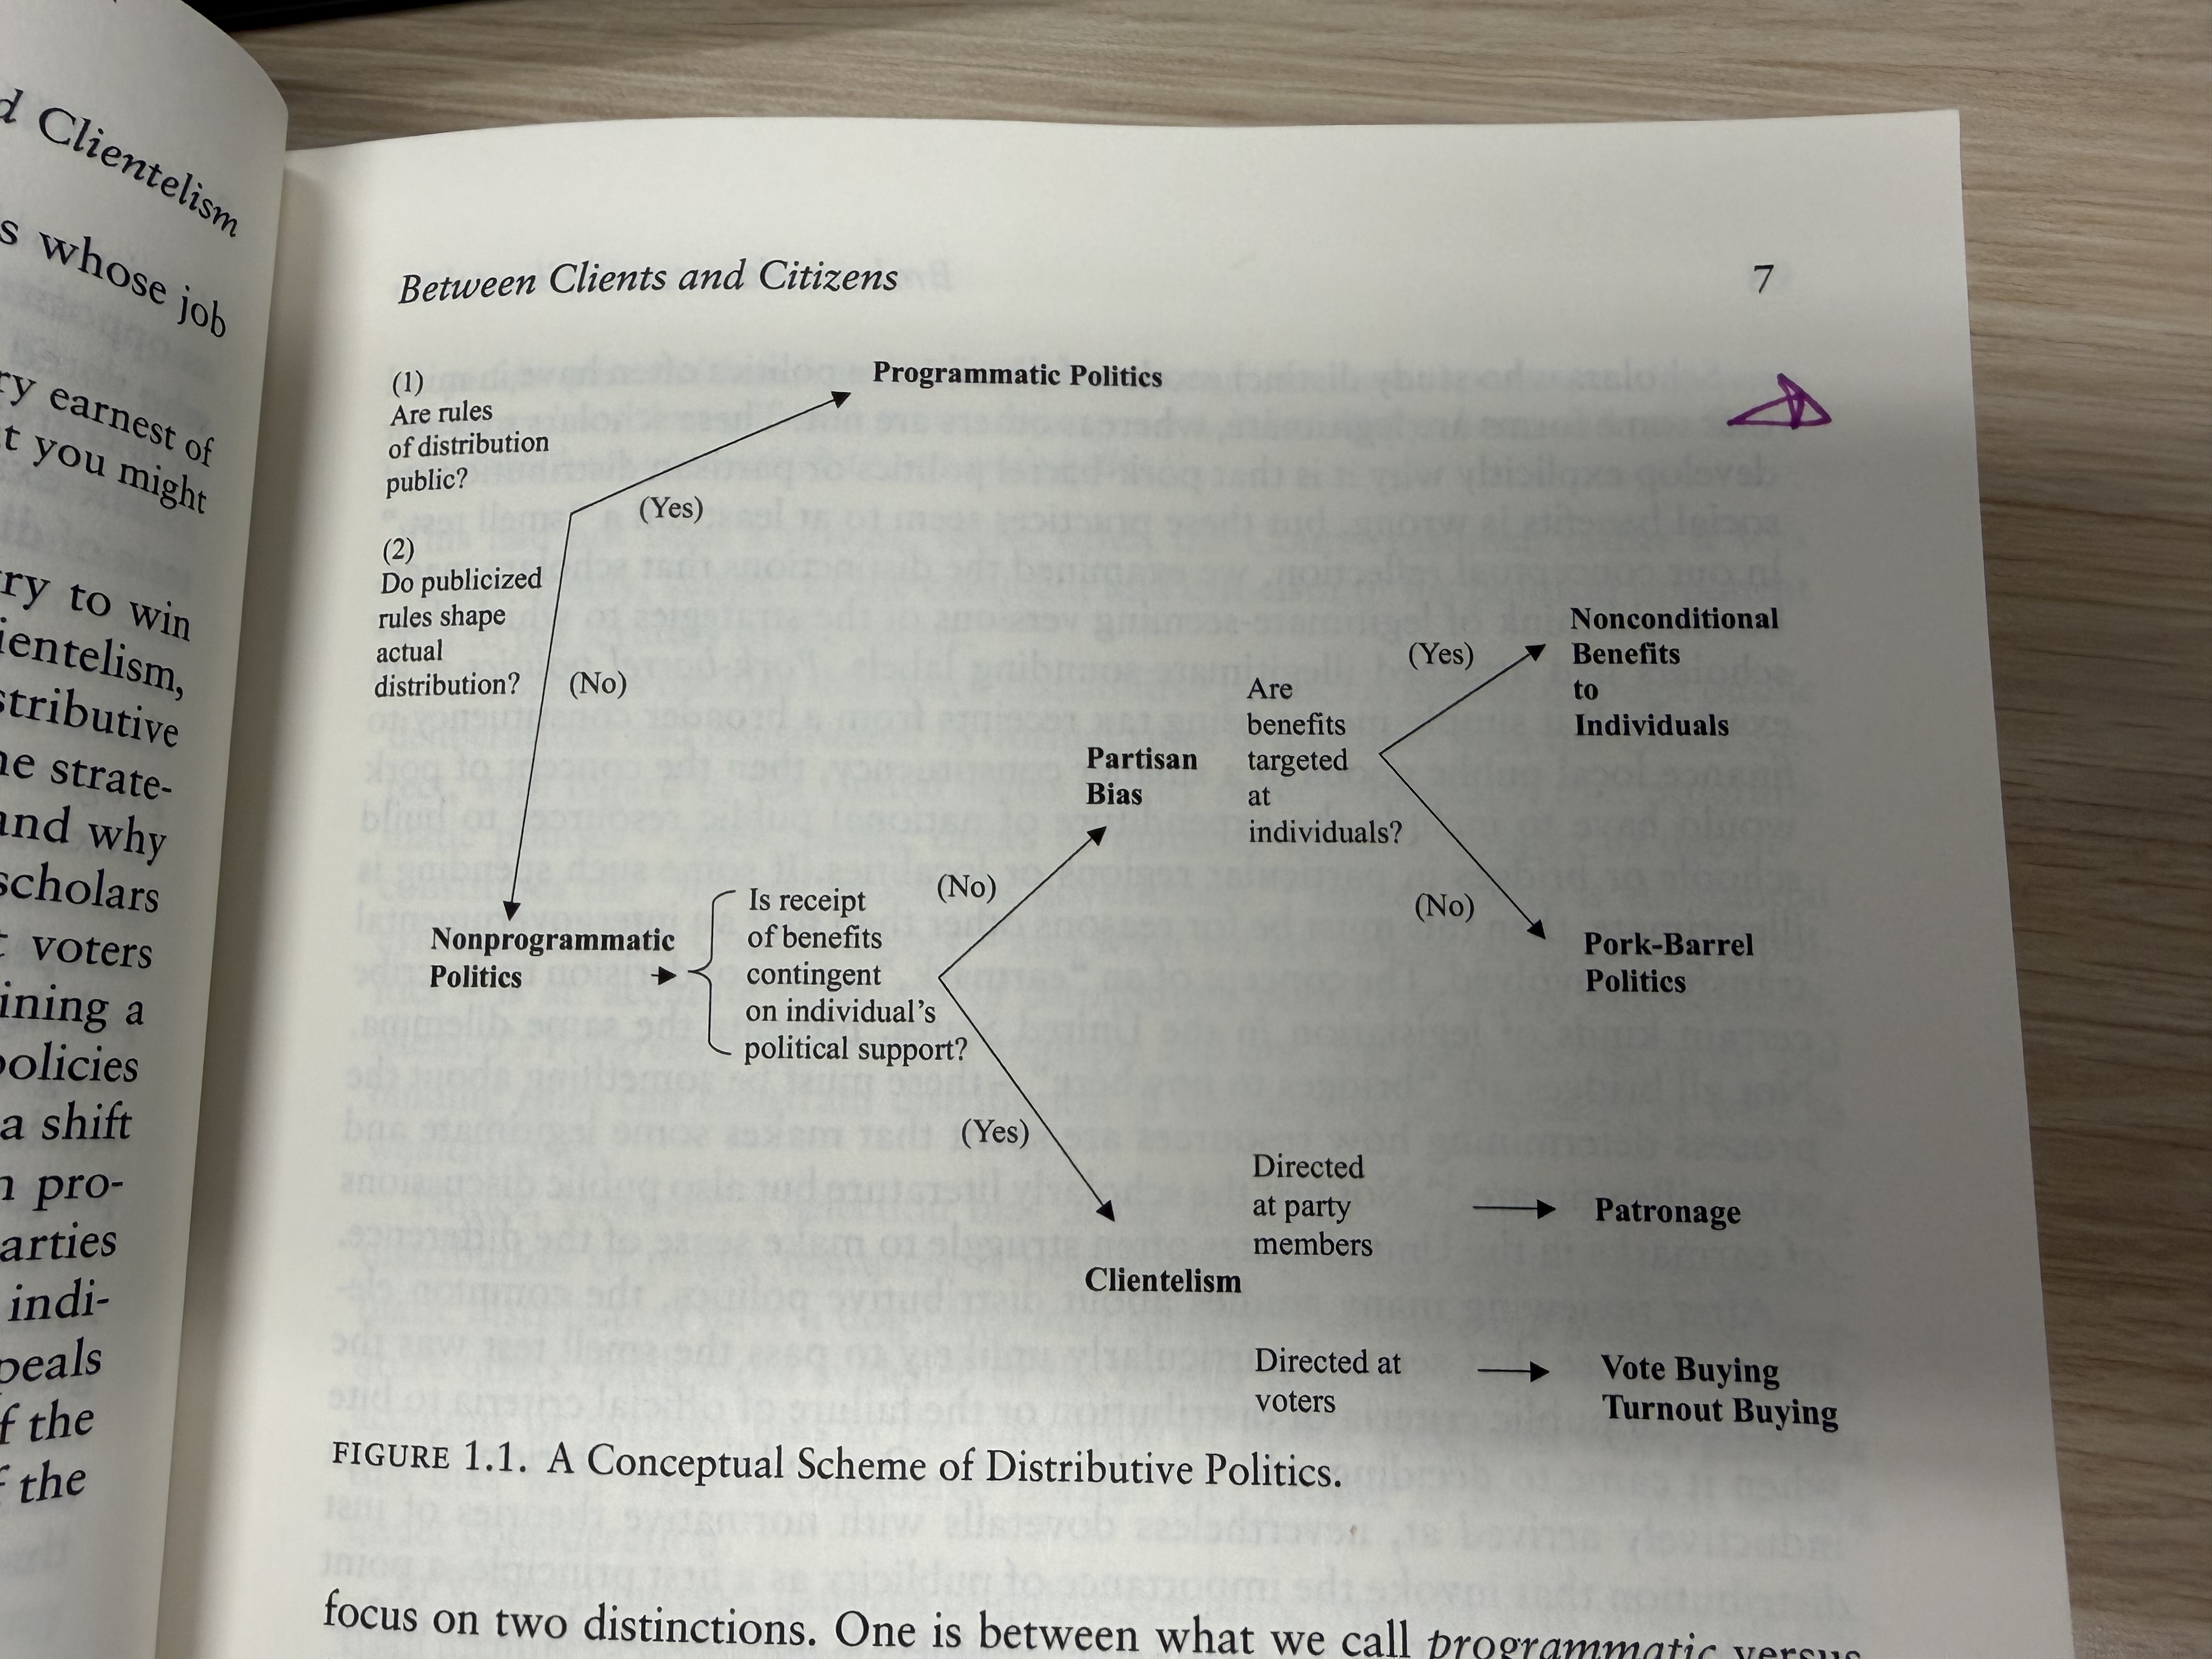
\includegraphics[width=14cm]{fig1.jpg}
    \end{center}
    \item A significant distinction (and in fact, the defining characteristic between programmatic and non-programmatic politics) is whether or not the rules (if followed) are public: is there some backdoor exchange, or is it a clear mechanism which simply funnels certain distribution? Note that this requires (or at least calls for) an institutional consideration: if there are not formal institutions shaping the redistributive process, then presumably there are also not actual rules publicly accessible and shaping said distribution. Per SCOTUS 1982:
    \begin{quote}
        ``We have never insisted that the franchise be exercised without tain of individual benefit; indeed, our tradition of political pluralism is partly predicated on the expectation that voters will pursue their individual good through the political process, and that the summation of these individual pursuits will further the collective welfare. So long as the hoped-for personal benefit is to be achieved through the normal processes of government, and not through some private arrangement, it always has been, and remains, a reputable basis upon which to cast one's ballot."
    \end{quote}
    \item Quid-pro-quo exchanges under clientilism are a normative threat: ``These exchanges seem to violate the free action or autonomy of voters. Even if we accept that voters are never fully autonomous and always come under the influence of some other actor -- parents, co-workers, ``opinion makers,'' or party leaders -- still the image of the voter being held to account for his or her choice is disquieting.''
    \item Clientelism requires an extraordinary amount of information regarding individual voters: their needs, their wants, their political leanings, and their ultimate political actions. The solution to this information problem is ``brokers,'' large quantitites of individuals employed by political machines to both gather and operate on this information. The broker is also tasked with providing specific benefits and actually implementing the ``get" side of distributive politica.Yet, by introducing brokers as contracted with political parties or centralized machines, we create a principal-agent tradeoff whereby there are potentially incentives to shirk or exploit. In short: vote buying works because of, and through, the political broker.
    \item Brokers have a clear incentive to target swing voters, and parties are not able to identify exactly who might be a swing voter versus safely support/opposition. Clientelism allows for these swing voters to be targeted by means of the broker's information and local expertise. Yet, empirically, this is not always true: in fact, swing voters are often under-represented in clientelism, while safe supporters tend to reap benefits at a disproportionate rate.
\end{itemize}


\section{Important Specific Factual Claims}

\begin{itemize}[leftmargin=*, itemsep=4pt]
    \item
\end{itemize}


\section{Connections}

\begin{itemize}
    \item Müller 1997: Discusses a transition away from party operatives/oganizations to instead surveys and mass media, particularly regarding socialist parties and mass movements in the mid-20th century. Presents a somewhat conflicting argument here (or at least, a different perspective in some cases) regarding whether or not the formal institution of the party itself is particularly relevant.
\end{itemize}


\section{My Critiques}

\begin{itemize}
    \item Less of a critique and more of a side point -- the work doesn't fully consider pressuring voters to abstain, either via intimidation or simply through general persuasive means. It may not be possible to convince dissidents to vote in line with the party, but it may be more feasible to convince them not to vote at all... (Addressed but only very briefly)
\end{itemize}


\end{document}
